\documentclass[grl]{agujournal2018}
%\documentclass[]{agujournal2018}
\usepackage{apacite}
\usepackage{natbib}

\usepackage{wrapfig}
\usepackage{url}
\usepackage{lineno}
\usepackage{trackchanges}
\soulregister\citet7
\soulregister\citep7
\soulregister\ref7
\addeditor{JKP} 


\draftfalse
\journalname{Geophysical Research Letters}

%custom packages
\usepackage{amsmath,amssymb,amsfonts,amsthm}
\usepackage{comment}
\usepackage{booktabs}
% custom commands
\newcommand\be{\begin{equation}}
\newcommand\ee{\end{equation}} 
\newcommand\bra{\langle}
\newcommand\ket{\rangle}
\newcommand\om{\omega}
\newcommand\tom{\tilde{\omega}}
\newcommand\tg{\tilde{g}}
\newcommand\tp{\tilde{p}}
\newcommand\tG{\tilde{G}}
\newcommand\El{\mathcal{L}}
%\usepackage{layouts}
%\printinunitsof{in}\prntlen{\textwidth} % check scales in the document
\linenumbers

% THIS IS THE LINENO PATCH TO WORK WITH AMSMATH
\newcommand*\patchAmsMathEnvironmentForLineno[1]{%
	\expandafter\let\csname old#1\expandafter\endcsname\csname #1\endcsname
	\expandafter\let\csname oldend#1\expandafter\endcsname\csname end#1\endcsname
	\renewenvironment{#1}%
	{\linenomath\csname old#1\endcsname}%
	{\csname oldend#1\endcsname\endlinenomath}}% 
\newcommand*\patchBothAmsMathEnvironmentsForLineno[1]{%
	\patchAmsMathEnvironmentForLineno{#1}%
	\patchAmsMathEnvironmentForLineno{#1*}}%
\AtBeginDocument{%
	\patchBothAmsMathEnvironmentsForLineno{equation}%
	\patchBothAmsMathEnvironmentsForLineno{align}%
	\patchBothAmsMathEnvironmentsForLineno{flalign}%
	\patchBothAmsMathEnvironmentsForLineno{alignat}%
	\patchBothAmsMathEnvironmentsForLineno{gather}%
	\patchBothAmsMathEnvironmentsForLineno{multline}%
}
% the patch comes from http://phaseportrait.blogspot.com/2007/08/lineno-and-amsmath-compatibility.html

\begin{document}



\title{Back to Einstein: burial-induced three-range diffusion in fluvial sediment transport}

\authors{J. Kevin Pierce \affil{1}and Marwan A. Hassan\affil{1}}
\affiliation{1}{Department of Geography \\University of British Columbia}
\correspondingauthor{Kevin Pierce}{kpierce@alumni.ubc.ca}

\begin{keypoints}
\item Random walk model describes coarse gravel tracers spreading out within a river as they gradually become buried
\item Interchange of grains between motion, surface rest, and burial states generates three diffusion ranges as the observation time increases
\item Sediment burial dominates long-time properties and exhumation may develop a fourth ``geomorphic'' range of tracer diffusion
\end{keypoints}

\begin{abstract}
Individual grains move through gravel bed rivers in cycles of motion and rest, so tracer grains diffuse as they transport downstream. Tracer experiments demonstrate at least three diffusion ranges as observation times increase, with different spreading rates in each range. Up till now, the generating processes of these ranges remains unclear. In this work, we develop a random walk model of individual bedload trajectories including motion, rest, and burial processes. The model describes three bedload diffusion ranges that terminate in a fourth non-diffusive range when all tracers become buried. Using the model, we attribute three-range tracer diffusion to the interplay between motion, rest, and burial processes, and we relate the multi-range diffusion characteristics to the timescales of these processes.
\end{abstract}

\section{Introduction}

Many environmental problems including channel morphology \citep{Hassan2017}, contaminant transport \citep{Macklin2006}, and aquatic habitat restoration \citep{Gaeuman2017} rely on our ability to predict the diffusion characteristics of coarse sediment tracers in river channels.
Diffusion is quantified by the time dependence of the positional variance $\sigma_x^2$ of a group of tracers.
With the scaling $\sigma_x^2 \propto t$, the diffusion is said to be normal, since this is found in the classic problems \citep{Taylor1920}.
However, with the scaling $\sigma_x^2 \propto t^\gamma$ with $\gamma \neq 1$, the diffusion is said to be anomalous \citep{Sokolov2012}, with $\gamma>1$ defining super-diffusion and $\gamma<1$ defining sub-diffusion \citep{Metzler2000}.
\citet{Einstein1937} developed one of the earliest models of bedload diffusion to describe a series of flume experiments \citep{Ettema2014}.
Interpreting individual bedload trajectories as a sequence of random steps and rests, Einstein originally concluded that a group of bedload tracers undergoes normal diffusion.

More recently, Nikora et al. realized coarse sediment tracers can show either normal or anomalous diffusion depending on the length of time they have been tracked \citep{Nikora2001a,Nikora2002}.
From numerical simulations and experimental data, Nikora et al. discerned ``at least three'' scaling ranges $\sigma_x^2 \propto t^\gamma$ as the observation time increased.
They associated the first range with ``local'' timescales less than the interval between subsequent collisions of moving grains with the bed, the second with ``intermediate'' timescales less than the interval between successive resting periods of grains, and the third with ``global'' timescales composed of many intermediate timescales.
Nikora et al. proposed super-diffusion in the local range, anomalous or normal diffusion in the intermediate range, and sub-diffusion in the global range.
They attributed these ranges to ``differences in the physical processes which govern the local, intermediate, and global trajectories'' of grains \citep{Nikora2001a}, and they called for a physically based model to explain the diffusion characteristics \citep{Nikora2002}.

Experiments support the Nikora et al. conclusion of multiple scaling ranges \citep{Martin2012,Fathel2016}, but they do not provide consensus on the expected number of ranges or their scaling properties.
This lack of consensus probably stems from resolution issues.
For example, experiments have tracked only moving grains, resolving the local range \citep{Furbish2012,Furbish2017,Fathel2016}; grains resting on the bed surface between movements, resolving the intermediate range \citep{Einstein1937,Yano1969,Nakagawa1976}; grains either moving or resting on the bed surface, likely resolving local and intermediate ranges \citep{Martin2012}; or grains resting on the surface after floods, likely resolving the global range \citep{Phillips2013,Bradley2017}. 
At long timescales, a significant fraction of tracers bury under the bed surface \citep{Hassan1991,Hassan2013,Ferguson2002a,Haschenburger2013,Papangelakis2016}, meaning burial dominates long term diffusion characteristics \citep{Bradley2017,Martin2014,Voepel2013}, possibly at global or even longer ``geomorphic'' timescales \citep{Hassan2017} than Nikora et al. originally considered.
As a result, three diffusion ranges can be identified by patching together multiple datasets \citep{Zhang2012,Nikora2002}, but they are not resolved by any one dataset.

Newtonian bedload trajectory models also show multiple diffusion ranges, although they also do not provide consensus on the expected number of ranges or their scaling properties. 
The majority of these models predict two ranges of diffusion (local and intermediate) without predicting a global range.
Among these, \citet{Nikora2001a} used synthetic turbulence \citep{Kraichnan1970} with a discrete element method for the granular phase \citep{Cundall1979}; \citet{Bialik2012} used synthetic turbulence with a random collision model \citep{Sekine1992}; and \citet{Fan2016} used a Langevin equation with probabilistic rests.
To our knowledge, only \citet{Bialik2015} have claimed to capture all three ranges from a Newtonian approach.
They incorporated a second resting mechanism into their earlier model \citep{Bialik2012}, implicitly suggesting that three diffusion ranges could result from two distinct timescales of sediment rest.
However, Newtonian approaches have not evaluated the effect of sediment burial on tracer diffusion, probably due to the long simulation timescales required. 

Random walk bedload diffusion models constructed in the spirit of \citet{Einstein1937} provide an alternative to the Newtonian approach and can include a second timescale of rest by incorporating sediment burial.
Einstein originally modeled bedload trajectories as instantaneous steps interrupted by durations of rest lying on statistical distributions \citep{Hassan1991}, but this generates only one range of normal diffusion \citep{Einstein1937,Hubbell1964,Nakagawa1976}.
Recently, researchers have generalized Einstein's model in a few different ways to describe multiple diffusion ranges.
\citet{Lisle1998} and \citet{Lajeunesse2018} promoted Einstein's instantaneous steps to motion intervals with random durations and a constant velocity, providing two diffusion ranges -- local and intermediate.
\citet{Wu2019} retained Einstein's instantaneous steps but included the possibility that grains can become permanently buried as they rest on the bed, also providing two diffusion ranges -- intermediate and global. 
These earlier works suggest the minimal required components to model three bedload diffusion ranges: (1) exchange between motion and rest intervals and (2) the sediment burial process.

In this study, we incorporate these two components into Einstein's original approach to describe three diffusion ranges with a physically based model, as called for by \citet{Nikora2002}.
Einstein was a giant in river geophysics and fostered an entire paradigm of research leveraging and generalizing his stochastic methods \citep{Hubbell1964, Yano1969, Yang1971, Gordon1972, Nakagawa1976,Paintal1971}.
Einstein's model can be viewed as a pioneering application of the continuous time random walk (CTRW) developed by \citet{Montroll1965} in condensed matter physics to describe the diffusion of charge carriers in solids.
To incorporate motion intervals and sediment burial, we utilize the multi-state CTRW developed by \citet{Weiss1976, Weiss1994} that extends the CTRW of \citet{Montroll1965}.
Below, we develop and solve the model in section \ref{sec:model}. Then, we discuss the predictions of our model, present its implications for local, intermediate, and global ranges of bedload diffusion, and suggest next steps for bedload diffusion research in sections \ref{sec:discussion} and \ref{sec:conclusion}.

\section{Bedload trajectories as a multi-state random walk}
\label{sec:model}
\subsection{Model assumptions}
\label{sec:assumptions}
We construct a three-state random walk where the states are motion, surface rest, and burial, and we label these states as $i=2$ (motion), $i=1$ (rest), and $i=0$ (burial).
Our target is the probability distribution $p(x,t)$ to find a grain at position $x$ and time $t$ if we know it started with the initial distribution $p(x,0)=\delta(x)$.
We characterize times spent moving or resting on the surface by exponential distributions $\psi_2(t)&=k_2e^{-k_2 t}$ and $\psi_1(t) &= k_1e^{-k_1t}$, since numerous experiments show thin-tailed distributions for these quantities \citep{Fathel2015,Roseberry2012,Einstein1937,Ancey2006,Martin2012}. We expect our conclusions will not be contingent on the specific distributions chosen, since all thin-tailed distributions provide similar diffusion characteristics in random walks \citep{Weiss1994,Weeks1998}.
We consider grains in motion to have characteristic velocity $v$ \citep{Lisle1998,Lajeunesse2018}, and we model burial as long lasting enough to be effectively permanent \citep{Wu2019}, with grains resting on the surface having a probability per unit time $\kappa$ to become buried, meaning $\Phi(t) = e^{-\kappa t}$ represents the probability that a grain is not buried after resting for a time $t$, while $1-\Phi(t)$ represents the probability that it is buried.
We specify the initial conditions with probabilities $\theta_1$ and $\theta_2$ to be in rest and motion at $t=0$, and we require $\theta_1+\theta_2=1$ for normalization.

\subsection{Governing equations}
Using these assumptions, we derive the governing equations for the set of probabilities $\om_{ij}(x,t)$ that a transition occurs from state $i$ to state $j$ at position $x$ and time $t$ using the statistical physics approach to multi-state random walks \citep{Weiss1994,Schmidt2007,Weeks1998}.
Denoting by $g_{ij}(x,t)$ the probability for a particle to displace by $x$ in a time $t$ within the state $i$ before it transitions to the state $j$, the transition probabilities $\om_{ij}(x,t)$ sum over all possible paths to the state $i$ from previous locations and times:
\be \om_{ij}(x,t) = \theta_i g_{ij}(x,t) + \sum_{k=0}^2 \int_0^x dx' \int_0^t dt' \om_{ki}(x',t')g_{ij}(x-x',t-t').\label{eq:g1}\ee
Defining another set of probabilities $G_i(x,t)$ that a particle displaces by a distance $x$ in a time $t$ within the state $i$ and possibly remains within the state, we perform a similar sums over paths for the probabilities to be in the state $i$ at $x$, $t$: 
\be p_i(x,t) = \theta_i G_i(x,t) + \sum_{k=0}^2 \int_0^x dx' \int_0^t dt' \om_{ki}(x',t')G_i(x-x',t-t').\label{eq:g2}\ee
Finally, the overall probability to be at position $x$ at time $t$ is
\be p(x,t) = \sum_{k=0}^2 p_k(x,t) \ee
This joint density is completely determined from the solutions of equations (\ref{eq:g1}-\ref{eq:g2}). We only need to specify the distributions $g_{ij}$ and $G_i$.


\subsection{Joint probability distribution}
\label{sec:solution}

We construct these distributions from the assumptions described in section \ref{sec:assumptions}.
Since particles resting on the bed surface bury in a time $t$ with probability $\Phi(t)$, and resting times are distributed as $\psi_1(t)$, we obtain $g_{12}(x,t) = \delta(x)k_1e^{-k_1t}e^{-\kappa t}$ and $g_{10}(x,t) = \delta(x) k_1 e^{-k_1 t}(1-e^{-\kappa t})$. Since motions have velocity $v$ for times distributed as $\psi_2(t)$, we have $g_{21}(x,t) = \delta(x-vt)k_2e^{-k_2 t}$.
Since burial is quasi-permanent, all other $g_{ij} = 0$.
The $G_i$ are constructed in the same way except using the cumulative probabilities $\int_t^\infty dt'\psi_i(t) = e^{-k_i t}$, since these characterize motions and rests that are ongoing \citep{Weiss1994}.
We obtain $G_1(x,t) = \delta(x)e^{-k_1t}$ and $G_2(x,t) = \delta(x-vt)e^{-k_2 t}$.

To solve equations (\ref{eq:g1}-\ref{eq:g2}) with these $g_{ij}$ and $G_i$, we take Laplace transforms in space and time $(x,t \rightarrow 
\eta,s) $ using a method similar to \citet{Weeks1998} to unravel the convolution structure of these equations, eventually obtaining
\be \tilde{p}(\eta,s) = \frac{1}{s}\frac{(s+\kappa + k')s  + \theta_1(s+\kappa )\eta v+ \kappa k_2}{(s+\kappa+k_1)\eta v+(s+\kappa+k')s + \kappa k_2}, \label{eq:nicedist}\ee
where $k' = k_1 + k_2$. Inverting this result using known Laplace transforms \citep{Prudnikov1986,Arfken1985} obtains
\begin{align}
\begin{split}
p(x,t) = \theta_1&\Big[1-\frac{k_1}{\kappa+k_1}\Big(1-e^{-(\kappa+k_1)t}\Big)\Big]\delta(x) \\ &+ \frac{1}{v}e^{-\Omega \tau - \xi}\Big(\theta_1\Big[k_1\mathcal{I}_0\big(2\sqrt{\xi\tau}\big) + k_2\sqrt{\frac{\tau}{\xi}}\mathcal{I}_1\big(2\sqrt{\xi\tau}\big)\Big] \\ 
&+ \theta_2\Big[k_1\delta(\tau) + k_2 \mathcal{I}_0\big(2\sqrt{\xi\tau}\big)+k_1 \sqrt{\frac{\xi}{\tau}}\mathcal{I}_1\big(2\sqrt{\xi\tau}\big)\Big]\Big) \\
&+ \frac{1}{v}\frac{\kappa k_2}{\kappa + k_1}e^{-\kappa \xi/(\kappa + k_1)}\Big[(\theta_1/\Omega)\mathcal{Q}_2(\xi/\Omega,\Omega\tau) + \theta_2 \mathcal{Q}_1(\xi/\Omega,\Omega\tau)\Big]
\label{eq:pdf}
\end{split}
\end{align}
for the joint distribution that a tracer is found at position $x$ at time $t$.
This result generalizes the earlier results of \citet{Lisle1998} and \citet{Einstein1937} to include sediment burial.
In this equation, we used the shorthand notations $\xi = k_2 x/v$, $\tau = k_1(t-x/v)$, and $\Omega = (\kappa+k_1)/k_1$ \citep{Lisle1998}. The $\mathcal{I}_\nu$ are modified Bessel functions of the first kind and the $\mathcal{Q}_\mu$ are generalized Marcum Q-functions defined by $\mathcal{Q}_\mu(x,y) = \int_0^y e^{-z-x}(z/x)^{(\mu-1)/2}\mathcal{I}_{\mu-1}(2\sqrt{xz})dz $ and originally devised for radar detection theory \citep{Marcum1960,Temme1996}. 
The Marcum Q-functions derive from the burial process.
Since we assumed resting grains could bury with an exponential probability while the resting probability follows a modified Bessel distribution \citep{Einstein1937,Lisle1998}, burial develops the Q-function convolution structure. 

\begin{figure}[t]
	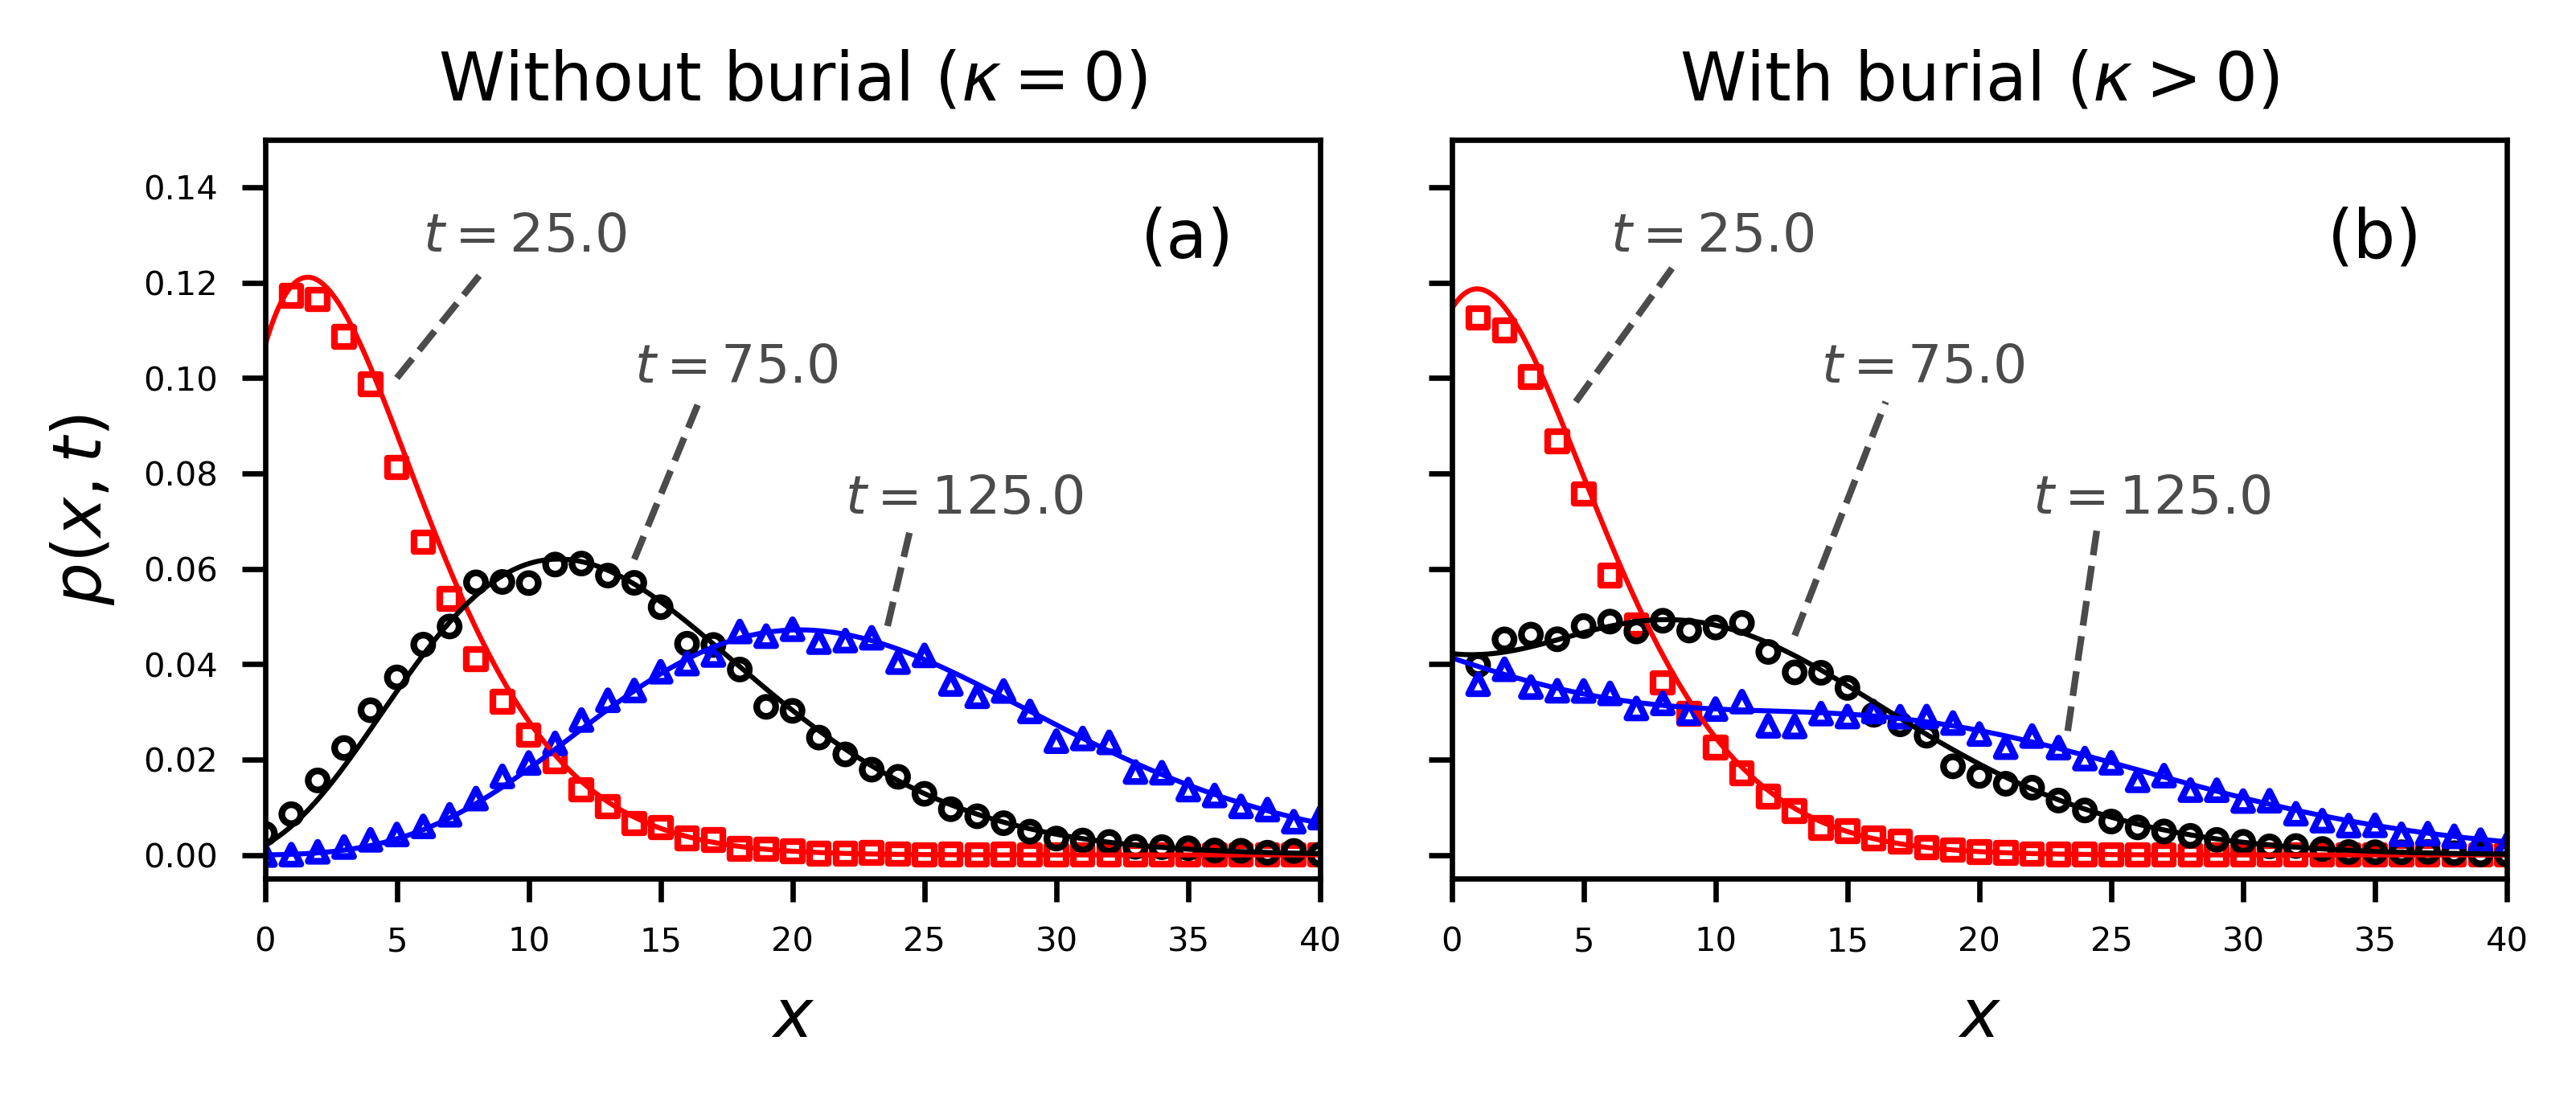
\includegraphics[width=\linewidth,keepaspectratio]{pdf-plot.png}
	\caption{Joint distributions for a grain to be at position $x$ at time $t$ are displayed for the choice $k_1=0.1$, $k_2=1.0$, $v=2.0$. Grains are considered initially at rest ($\theta_1=1$, $\theta_2=0$). The solid lines are the analytical distribution in equation (\ref{eq:pdf}), while the points are numerically simulated, showing the correctness of our derivations. Colors pertain to different times. Units are unspecified, since we aim to demonstrate the general characteristics of $p(x,t)$. Panel (a) shows the case $\kappa=0$ -- no burial. In this case, the joint distribution tends toward Gaussian at large times \citep{Einstein1937,Lisle1998}. Panel (b) shows the case when grains have rate $\kappa = 0.01$ to become buried while resting. Because of burial, the joint distribution tends toward a more uniform distribution than Gaussian.
	\label{fig:pdfs}}
\end{figure}

Figure \ref{fig:pdfs} depicts the distribution (\ref{eq:pdf}) alongside simulations generated by a direct method based on evaluating the cumulative transition probabilities between states on a small timestep \citep{Barik2006}.
When grains do not become buried, as in panel (a) of figure \ref{fig:pdfs}, the distribution becomes Gaussian-like at relatively large observation times, exemplifying normal diffusion and satisfying the central limit theorem.
When grains become buried, as in panel (b) of figure \ref{fig:pdfs},  the Q-function terms prevent the distribution from approaching a Gaussian at large timescales, exemplifying anomalous diffusion \citep{Weeks1998} and violating the central limit theorem \citep{Metzler2000,Schumer2009}.


\subsection{Positional variance}

To obtain an analytical formula for tracers diffusing downstream while they gradually become buried, we derive the first two moments of position by taking derivatives with respect to $\eta$ of the Laplace space distribution (\ref{eq:nicedist}) using an approach similar to \citet{Shlesinger1974} and \citet{Weeks1998}, and we use these to calculate the positional variance $\sigma_x^2 = \bra x^2\ket - \bra x \ket^2$. 
The first two moments are
\begin{align}
\bra x(t) \ket &= A_1 e^{(b-a)t}+B_1e^{-(a+b)t}+C_1, \label{eq:mean}\\
\bra x^2(t) \ket &= A_2(t)e^{(b-a)t}+B_2(t)e^{-(a+b)t}+C_2, \label{eq:second}
\end{align}
so the variance is 
\be \sigma_x^2(t) = A(t)e^{(b-a)t} + B(t)e^{-(a+b)t} + C(t). \label{eq:var}\ee
In these equations, $a = (\kappa + k_1+k_2)/2$ and $b = \sqrt{a^2-\kappa k_2}$ are effective rates having dimensions of inverse time, while the $A$, $B$, and $C$ factors are provided in table \ref{table:params}.

%\\
%		&\hspace{1cm}
\begin{table}[!h]
	\centering
%\begin{wraptable}{r}{width=5.5cm}
	\caption{Abbreviations used in the expressions of the mean (\ref{eq:mean}), second moment (\ref{eq:second}) and variance (\ref{eq:var}) of bedload tracers.}
	\label{table:params}
\small
	\begin{tabular}{c}
		\toprule
		$\begin{aligned}[t]
		&A_1 = \frac{v}{2b}\big[\theta_2+\frac{k_1+\theta_2\kappa}{b-a}\big] \\
		&B_1 = -\frac{v}{2b}\big[\theta_2-\frac{k_1+\theta_2 \kappa}{a+b}\big] \\
		&C_1 =  -\frac{v}{2b}\big[\frac{k_1+\theta_2 \kappa}{b-a}+\frac{k_1+\theta_2 \kappa}{a+b}\big]\\
		&A_2(t) = \frac{v^2}{2b^3}\Big[(bt-1)[k_1+\theta_2(2\kappa + k_1 + b-a)]+\theta_2b 
		 + \frac{(\kappa+k_1)(\theta_2\kappa+k_1)}{(b-a)^2}[(bt-1)(b-a)-b]\Big]\\
		&B_2(t) = \frac{v^2}{2b^3}\Big[(bt+1)[k_1 + \theta_2(2\kappa+k_1-a-b)]+\theta_2b
		 -\frac{(\kappa+k_1)(\theta_2\kappa+k_1)}{(a+b)^2}[(bt+1)(a+b)+b]\Big]\\
		&C_2 = \frac{v^2}{2b^3}(\kappa+k_1)(\theta_2 \kappa + k_1)\Big[\frac{2b-a}{(b-a)^2}+\frac{a+2b}{(a+b)^2}\Big]\\
		&A(t) = A_2(t)-2A_1C_1 - A_1^2\exp[(b-a)t]\\
		&B(t) = B_2(t)-2B_1C_1 - B_1^2\exp[-(a+b)t]\\
		&C(t) = C_2-C_1^2-2A_1B_1\exp[-2at]\\			
		\end{aligned}$\\
		\bottomrule
	\end{tabular}
%\end{wraptable}
\vspace{-0.5cm}
\end{table}
The positional variance (\ref{eq:var}) is plotted in figure \ref{fig:var} for conditions $\theta_1=1$ and $k_2\gg k_1 \gg \kappa$.
We interpret ``$\gg$'' to mean ``of at least an order of magnitude greater''.
These conditions are most relevant to tracers in gravel-bed rivers, since they represent that grains are initially at rest \citep{Hassan1991,Wu2019}, motions are typically much shorter than rests \citep{Einstein1937,Hubbell1964}, and burial requires a much longer time than typical rests  \citep{Ferguson2002,Hassan1994,Haschenburger2013}.
Figure \ref{fig:var} demonstrates that under these conditions the variance (\ref{eq:var}) shows three diffusion ranges with approximate power law scaling ($\sigma_x^2 \propto t^\gamma$) that we identify as the local, intermediate, and global ranges proposed by Nikora et al., followed by a fourth range of no diffusion ($\sigma_x^2 = \text{const}$) stemming from the burial of all tracers. 
We suggest to call the fourth range geomorphic, since any further transport in this range can occur only if scour re-exposes buried grains to the flow \citep{Nakagawa1980,Voepel2013,Martin2014,Wu2019a}.

\begin{figure}[h!]	
	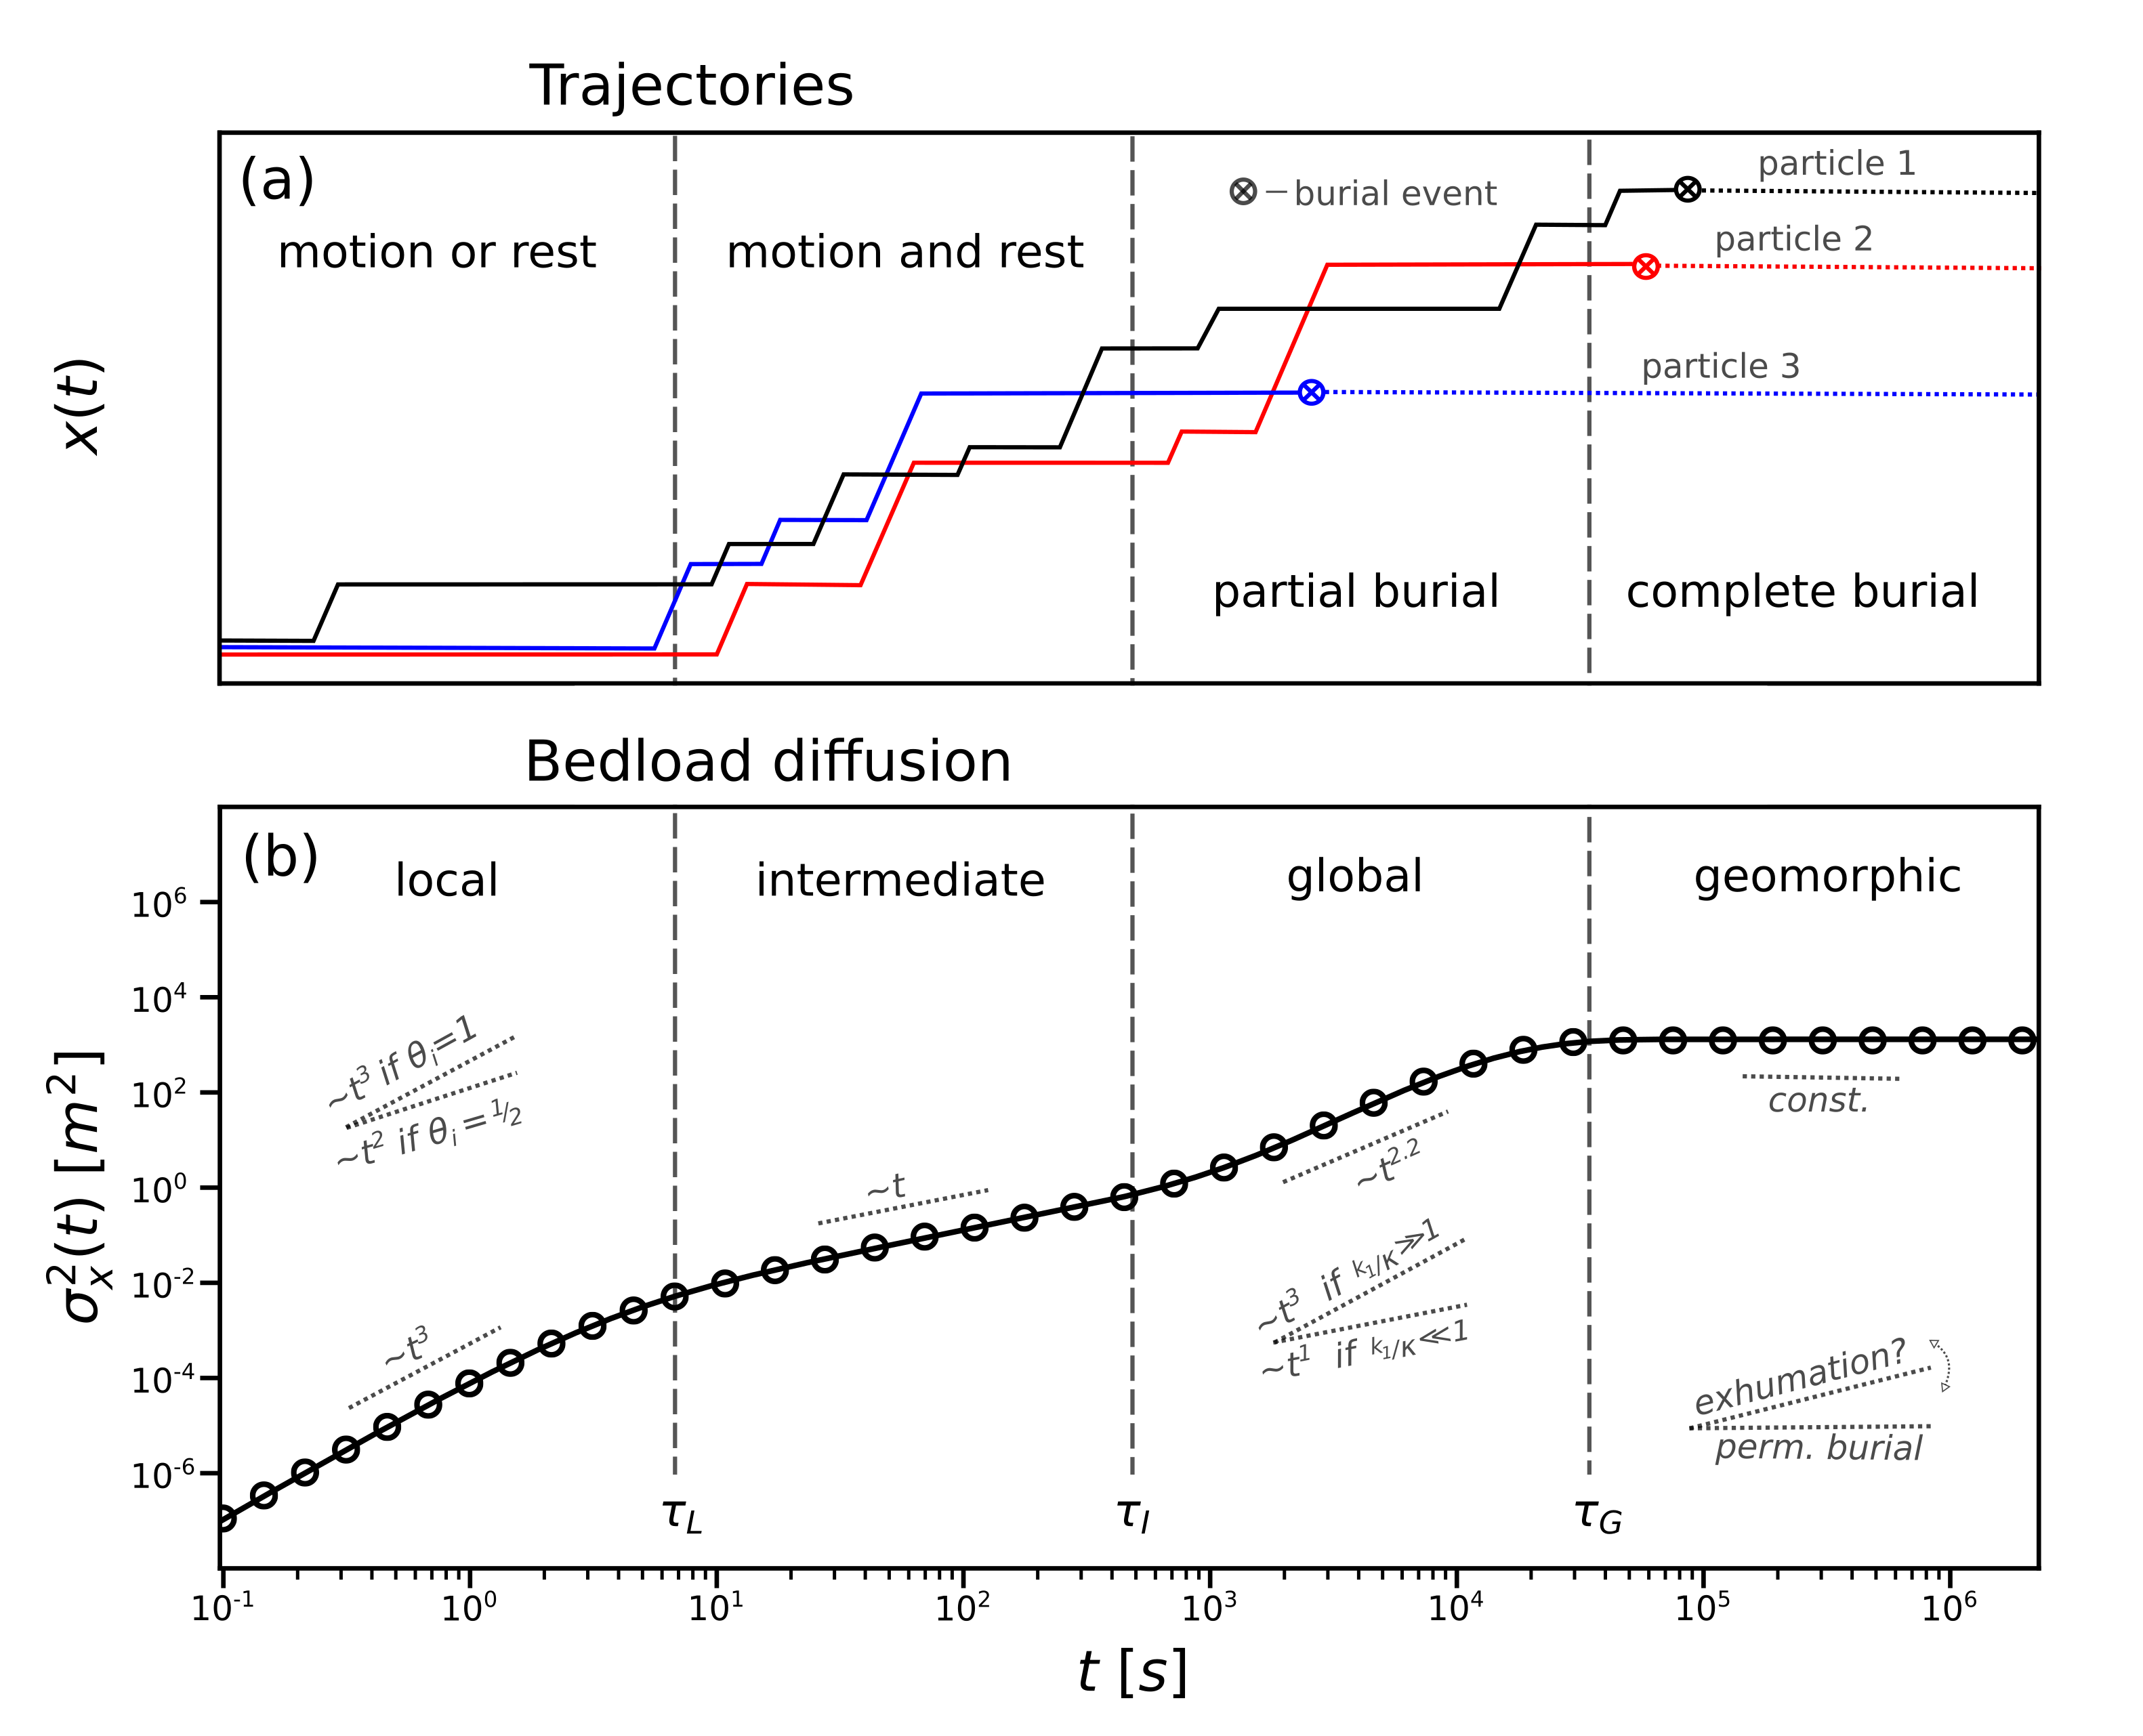
\includegraphics[width=\linewidth,keepaspectratio]{diffusion.png}
	\caption{Panel (a) sketches conceptual trajectories of three grains, while panel (b) depicts the variance (\ref{eq:var}) with mean motion time $1.5$ s, resting time $30.0$ s, and movement velocity $0.1$ m/s -- values comparable to laboratory experiments transporting small ($5$ mm) gravels \citep{Lajeunesse2010,Martin2012}. The burial timescale is $7200.0$s (two hours), and grains start from rest ($\theta_1=1$). The solid line is equation (\ref{eq:var}), and the points are numerically simulated. Panel (b) demonstrates four distinct scaling ranges of $\sigma_x^2$: local, intermediate, global, and geomorphic. The first three are diffusive. Three crossover times $\tau_L$, $\tau_I$, and $\tau_G$ divide the ranges. Within each range, a slope key demonstrates the scaling $\sigma_x^2 \propto t^\gamma$. Panel (a) demonstrates that different mixtures of motion, rest, and burial states generate the ranges. At local timescales, grains usually either rest or move; at intermediate timescales, they transition between rest and motion; at global timescales, they transition between rest, motion, and burial; and at geomorphic timescales, all grains bury. Additional slope keys in the local and global ranges of panel (b) illustrate the effect of initial conditions and rest/burial timescales on the diffusion, while the additional slope key within the geomorphic range demonstrates the expected scaling when burial is not permanent, as we discuss in section \ref{sec:discussion}.
}
	\label{fig:var}
\end{figure}

\subsection{Diffusion exponents}

Two limiting cases of equation (\ref{eq:var}) provide the scaling exponents $\gamma$ of the diffusion $\sigma_x^2 \propto t^\gamma$ in each range. Limit (1) represents times so short a negligible amount of sediment burial has occurred, $t\ll 1/\kappa$, while limit (2) represents times so long motion intervals appear as instantaneous steps of mean length $l=v/k_2$, $1/k_2 \rightarrow 0$ while $v/k_2 = \text{constant}$.
Limit (1) provides local exponent $2 \leq \gamma \leq 3$ depending on the initial conditions $\theta_i$, and intermediate exponent $\gamma=1$.
If grains start in motion or rest exclusively, meaning one $\theta_i = 0$, the local exponent is $\gamma=3$, while if grains start in a mixture of motion and rest states, meaning neither $\theta_i$ is zero, the local exponent is $\gamma=2$.
Limit (2) provides global exponent $1 \leq \gamma \leq 3$ depending on the relative importance of $\kappa$ and $k_1$.
In the extreme $k_1/\kappa \ll 1$, we find $\gamma=1$ in the global range, while in the opposite extreme $k_1/\kappa \rightarrow \infty$ we find $\gamma=3$.
We summarize when $k_2\gg k_1 \gg \kappa$ so all three diffusion ranges exist, equation (\ref{eq:var}) implies:
\begin{enumerate}
\item local range super-diffusion with $2<\gamma<3$ depending on whether grains start from purely motion or rest ($\gamma=3$) or from a mixture of both states ($\gamma=2$),
\item intermediate range normal diffusion $\gamma=1$ independent of model parameters, and
\item global range super-diffusion $1<\gamma<3$ depending on whether burial happens relatively slowly ($\gamma \rightarrow 1$) or quickly ($\gamma \rightarrow 3$) compared to surface resting times.
\end{enumerate}
Finally, the burial of all tracers generates a geomorphic range of no diffusion.

\section{Discussion}
\label{sec:discussion}

\subsection{Local and intermediate ranges with comparison to earlier work}

We extended \citet{Einstein1937} by including motion and burial processes in a multi-state random walk \citep{Weiss1994,Weeks1998} to demonstrate that a group of bedload tracers moving downstream while gradually becoming buried will generate a super-diffusive local range \citep{Martin2012,Fathel2016,Witz2018}, a normal-diffusive intermediate range \citep{Nakagawa1976,Yano1969}, and a super-diffusive global range \citep{Bradley2017, Bradley2010}, before the diffusion eventually terminates in a geomorphic range \citep{Hassan2017}.
\citet{Nikora2002} highlighted the need for such a physical description, although they suggested to use a two-state random walk between motion and rest states with heavy-tailed resting times, and they did not discuss sediment burial.
However, other works have demonstrated that a two-state walk with heavy-tailed rests provides two diffusion ranges -- not three \citep{Weeks1996,Fan2016}, and although heavy-tailed resting times have been documented for surface particles \citep{Liu2019,Fraccarollo2019}, they are more often associated with buried particles \citep{Martin2012,Martin2014,Voepel2013,Olinde2015,Pelosi2016, Pierce2020}, while surface particles retain light-tailed resting times \citep{Einstein1937,Yano1969,Ancey2006,Nakagawa1976}.
Accordingly, we developed a random walk model of bedload trajectories with light-tailed surface resting times that incorporates sediment burial.

The local and intermediate range diffusion characteristics resulting from our model correspond closely to the original Nikora et al. concepts, while our global range has a different origin than Nikora et al. envisioned.
\citet{Nikora2001a} explained that local diffusion results from the non-fractal (smooth) characteristics of bedload trajectories between subsequent interactions with the bed,  while intermediate diffusion results from the fractal (rough) characteristics of bedload trajectories after many interactions with the bed.
Our model represents these conclusions: non-fractal (and super-diffusive) bedload trajectories exist on timescales short enough that each grain is either resting or moving, while fractal (and normal-diffusive) bedload trajectories exist on timescales when grains are actively switching between motion and rest states.
We conclude that local and intermediate ranges stem from the interplay between motion and rest timescales, as demonstrated by earlier two-state random walk models \citep{Lisle1998,Lajeunesse2018} and by all Newtonian models that develop sequences of motions and rests \citep{Nikora2001a, Bialik2012}, even those including heavy-tailed rests \citep{Fan2016}. 

\subsection{Global and geomorphic ranges with next steps for research}

Nikora et al. explained that divergent resting times generate a sub-diffusive global range.
However, studies have demonstrated that divergent resting times can generate super-diffusion in asymmetric random walks \citep{Weeks1996,Weeks1998}, and both experiments \citep{Bradley2017,Bradley2010} and models \citep{Pelosi2016,Wu2019,Wu2019a} of bedload tracers undergoing burial have demonstrated global range super-diffusion.
While our results also show global range super-diffusion, they do not necessarily refute the Nikora et al. conclusion of sub-diffusion at long timescales.
We assumed sediment burial was a permanent condition which developed a non-diffusive geomorphic range.
In actuality, burial is a temporary condition, because bed scour can exhume buried sediment back into transport \citep{Wu2019a}, probably after heavy-tailed intervals \citep{Voepel2013,Martin2014,Pierce2020}.
We anticipate that a generalization of our model to include heavy-tailed timescales between burial and exhumation would develop four ranges of diffusion, where the long-time decay of the exhumation time distribution would dictate the geomorphic range diffusion characteristics as depicted in figure \ref{fig:var}.
If cumulative exhumation times decay faster than $T^{-1/2}$, as suggested by equilibrium transport models \citep{Voepel2013, Martin2014, Pierce2020} and laboratory experiments \citep{Martin2014,Martin2012}, we expect a super-diffusive geomorphic range \citep{Weeks1998}.
However, if they decay slower than $T^{-1/2}$, as implicitly suggested by the data of \citet{Olinde2015}, we expect a genuinely sub-diffusive geomorphic range \citep{Weeks1998}, leaving Nikora et al. with the final word on long-time sub-diffusion.

The analytical solution of bedload diffusion in equation (\ref{eq:var}) reduces exactly to the analytical solutions of the \citet{Lisle1998} and \citet{Lajeunesse2018} models in the limit without burial ($\kappa \rightarrow 0$), the \citet{Wu2019} model in the limit of instantaneous steps ($k_2 \rightarrow \infty$ and $l = v/k_2$), and the original \citet{Einstein1937} model in the limit of instantaneous steps without burial.
These reductions demonstrate that the majority of recent bedload diffusion models, whether developed from Exner-type equations \citep{Wu2019,Pelosi2014,Pelosi2016} or advection-diffusion equations \citep{Lisle1998,Lajeunesse2018}, can be viewed equivalently as continuous-time random walks applied to individual bedload trajectories.
Within random walk theory, sophisticated descriptions of transport with variable velocities \citep{Zaburdaev2008,Masoliver1994}, correlated motions \citep{Escaff2018,Vicsek2012a}, and anomalous diffusion \citep{Masoliver2016,Fa2014,Metzler2014} have been developed.
Meanwhile, in bedload transport research, variable velocities \citep{Lajeunesse2010,Furbish2012,Heyman2016}, correlated motions \citep{Heyman2014,Lee2018,Saletti2020}, and anomalous diffusion \citep{Fathel2016,Bradley2017,Schumer2009} constitute open research issues.
We believe further developing the linkage between existing bedload models and random walk concepts could rapidly progress our understanding.

\section{Conclusion}
\label{sec:conclusion}
We developed a random walk model to describe sediment tracers transporting through a river channel as they gradually become buried, providing a physical description of the local, intermediate, and global diffusion ranges identified by \citet{Nikora2002}.
Pushing their ideas somewhat further, we proposed a geomorphic range to describe diffusion characteristics at timescales larger than the global range when burial and exhumation both moderate downstream transport.
At base level, our model demonstrates that (1) durations of sediment motions, (2) durations of sediment rest, and (3) the sediment burial process are sufficient to develop three diffusion ranges that terminate when all tracers become buried.
A next step is to incorporate exhumation to better understand the geomorphic range.
Ultimately, we emphasize that the multi-state random walk formalism used in this paper implicitly underlies most existing bedload diffusion models and provides a powerful tool for researchers targeting landscape-scale understanding from statistical concepts of the underlying grain-scale dynamics.

\appendix


\acknowledgments
K. Pierce acknowledges thoughtful exchanges with Eduardo Daly and Eric Weeks during the early stages of this work. Both authors would like to thank Matteo Saletti, Conor McDowell, Shawn Chartrand, and Will Booker for helpful discussions. M. Hassan is supported by an NSERC Discovery grant. The Python simulation code is freely available at \sloppy
\url{https://zenodo.org/record/3659291#.Xj3p7XVKjIU}.

\bibliography{biblio.bib}
\end{document}
